\documentclass[13pt,oneside]{book}
\usepackage[utf8]{inputenc}
\usepackage{url}
\usepackage{graphicx}

\usepackage{geometry}
\geometry{a4paper, left=20mm, right=20mm, top=20mm, bottom=20mm}
\usepackage[margin=1.2in]{geometry}
\usepackage[toc,page]{appendix}
\usepackage{graphicx}
\usepackage{natbib}
\usepackage{lipsum}
\usepackage{caption}

\begin{document}

\captionsetup[figure]{margin=1.5cm,font=small,labelfont={bf},name={Figure},labelsep=colon,textfont={it}}
\captionsetup[table]{margin=1.5cm,font=small,labelfont={bf},name={Table},labelsep=colon,textfont={it}}
\setlipsumdefault{1}

\begin{titlepage}
\begin{center}
{\LARGE College Of Engineering Trivandrum}\\[3cm]
\linespread{1.2}\huge {\bfseries Application Software Development Lab}\\[3cm]
\linespread{1}

\includegraphics[width=5cm]{img/emblem.jpeg}\\[3cm]
{\Large Gokul K\\ S5  CSE \\ Roll No:21\\ TVE18CS021 }\\[1cm]


\textit{ }\\[2cm]
Department of Computer Science\\[0.2cm]
\today
\end{center}

\end{titlepage}

\newpage
\large
\noindent{\bfseries{\huge Contents}\hfill Page No.\vspace \bigskipamount \par }
\contentsline {chapter}{\numberline {1}Basics of SQL}{3}
\contentsline {section}{\numberline {1.1}Aim}{3}
\contentsline {section}{\numberline {1.2}Theory}{3}
\contentsline {section}{\numberline {1.3}Experiment}{4}
\contentsline {section}{\numberline {1.4}Result}{7}
\contentsline {chapter}{\numberline {2}Basic SQL Queries - I}{8}
\contentsline {section}{\numberline {2.1}Aim}{8}
\contentsline {section}{\numberline {2.2}Experiment}{8}
\contentsline {section}{\numberline {2.3}Result}{12}
\contentsline {chapter}{\numberline {3}Basic SQL Queries - II}{13}
\contentsline {section}{\numberline {3.1}Aim}{13}
\contentsline {section}{\numberline {3.2}Experiment}{13}
\contentsline {section}{\numberline {3.3}Result}{19}
\contentsline {chapter}{\numberline {4}Introduction to Aggregate functions}{20}
\contentsline {section}{\numberline {4.1}Aim}{20}
\contentsline {section}{\numberline {4.2}Theory}{20}
\contentsline {section}{\numberline {4.3}Experiment}{20}
\contentsline {section}{\numberline {4.4}Result}{25}
\contentsline {chapter}{\numberline {5}Data Constraints and Views}{26}
\contentsline {section}{\numberline {5.1}Aim}{26}
\contentsline {section}{\numberline {5.2}Theory}{26}
\contentsline {section}{\numberline {5.3}Experiment}{26}
\contentsline {section}{\numberline {5.4}Result}{31}
\contentsline {chapter}{\numberline {6}String Functions and Pattern Matching}{32}
\contentsline {section}{\numberline {6.1}Aim}{32}
\contentsline {section}{\numberline {6.2}Theory}{32}
\contentsline {section}{\numberline {6.3}Experiment}{33}
\contentsline {section}{\numberline {6.4}Result}{39}
\contentsline {chapter}{\numberline {7}Join Statements, Set Operations, Nested Queries and Grouping}{40}
\contentsline {section}{\numberline {7.1}Aim}{40}
\contentsline {section}{\numberline {7.2}Theory}{40}
\contentsline {section}{\numberline {7.3}Experiment}{40}
\contentsline {section}{\numberline {7.4}Result}{47}
\contentsline {chapter}{\numberline {8}PL/SQL and Sequence}{48}
\contentsline {section}{\numberline {8.1}Aim}{48}
\contentsline {section}{\numberline {8.2}Theory}{48}
\contentsline {section}{\numberline {8.3}Experiment}{48}
\contentsline {section}{\numberline {8.4}Result}{54}
\contentsline {chapter}{\numberline {9}Cursor}{55}
\contentsline {section}{\numberline {9.1}Aim}{55}
\contentsline {section}{\numberline {9.2}Theory}{55}
\contentsline {section}{\numberline {9.3}Experiment}{55}
\contentsline {section}{\numberline {9.4}Result}{59}
\contentsline {chapter}{\numberline {10}Trigger and Exception Handling}{60}
\contentsline {section}{\numberline {10.1}Aim}{60}
\contentsline {section}{\numberline {10.2}Theory}{60}
\contentsline {section}{\numberline {10.3}Experiment}{60}
\contentsline {section}{\numberline {10.4}Result}{69}
\contentsline {chapter}{\numberline {11}Procedures, Functions and Packages}{70}
\contentsline {section}{\numberline {11.1}Aim}{70}
\contentsline {section}{\numberline {11.2}Theory}{70}
\contentsline {section}{\numberline {11.3}Experiment}{70}
\contentsline {section}{\numberline {11.4}Result}{75}
\newpage

\begin{frame}{}
    \centering
    \hspace*{-0.5cm}
    $\vcenter{\hbox{
\includegraphics[width=1.5cm]{img/emblem.jpeg}}}$
    $\vcenter{\resizebox{0.95\textwidth}{!}{
        \begin{tabular}{c}
             CS333 - Application Software Development Lab $\cdot$ 2020 $\cdot$   \\
             \hline 
        \end{tabular}
    }}$
\end{frame}
\section*{Cycle 1}
\section*{Expt 1}
\begin{center}
    \Large{Basic SQL Queries - I}
\end{center}

\section*{Aim}
\large{Creation of a database using DDL commands
	\begin{enumerate}
		\item Create Table
		\item Alter Table
		\item Truncate Table
		\item Drop Table
	\end{enumerate}
}
\section*{Theory}
SQL statements are divided into these categories:\\
1.Data Definition Language (DDL) Statements\\
2.Data Manipulation Language (DML) Statements\\
3.Transaction Control Statements (TCL)\\
4.Session Control Statement\\
5.System Control Statement\\
\textbf{Managing tables}\\
A table is the data structure that holds data in a relational database. A table is
composed of rows and columns.
A table can represent a single entity that you want to track within your system.
This type of a table could represent a list of the employees within your organization,
or the orders placed for your company’s products.
A table can also represent a relationship between two entities. This type of a
table could portray the association between employees and their job skills, or the
relationship of products to orders. Within the tables, foreign keys are used to represent
relationships.\\
\textbf{Creating Tables}\\
To create a table, use the SQL command CREATETABLE.
Syntax:\\
CREATE TABLE ’TABLE NAME’(’FIELD NAME ’ ’DATA TYPE’ ’SIZE’,..........)\\
\textbf{Altering Tables}\\
1. To add one or more new columns to the table\\
2. To add one or more integrity constraints to a table\\
3. To modify an existing column’s definition (datatype, length, default value, and
NOTNULL integrity constraint)\\
4. To modify data block space usage parameters (PCTFREE, PCTUSED)\\
5. To modify transaction entry settings (INITRANS, MAXTRANS)\\
6. To modify storage parameters (NEXT, PCTINCREASE, etc.)\\
7. To enable or disable integrity constraints associated with the table\\
8. To drop integrity constraints associated with the table
\section*{Experiment}
	\begin{enumerate}
		\item 
			Create a table named EMPLOYEE \\
			Syntax:
			\begin{verbatim}
				CREATE TABLE EMPLOYEE (
					EMPNO INTEGER(4) PRIMARY KEY,
					ENAME VARCHAR(10),
					DESIGNATION VARCHAR(10),
					SALARY DECIMAL(8, 2)
				);
				DESC EMPLOYEE;
			\end{verbatim}
			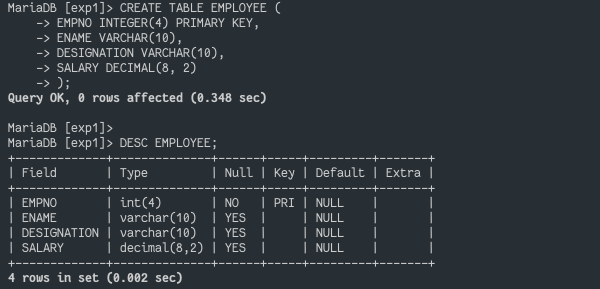
\includegraphics{img/p1/ss1.png}
		
			\item 
			a) Alter the table by adding column QUALIFICATION. \\
			b) Alter the table by modifying the EMPNO size to 6. \\
			c) Rename the table EMPLOYEE to EMP\_NEW. \\
			d) Drop the column QUALIFICATION.\\
			Syntax:
			\begin{verbatim}
				ALTER TABLE EMPLOYEE
				ADD QUALIFICATION VARCHAR(10);

				DESC EMPLOYEE;
			\end{verbatim}
			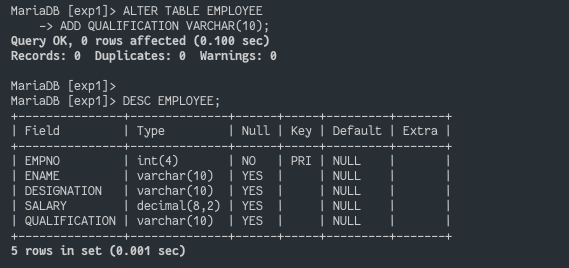
\includegraphics{img/p1/ss2.png}
			\begin{verbatim}
				ALTER TABLE EMPLOYEE
				MODIFY COLUMN EMPNO INTEGER(6);

				DESC EMPLOYEE;
			\end{verbatim}
			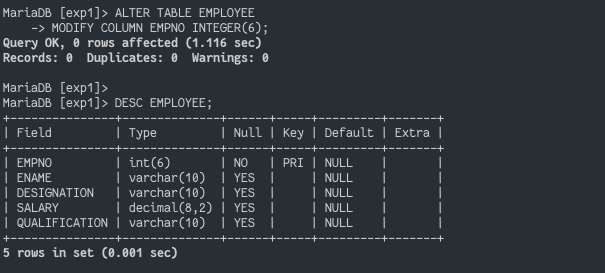
\includegraphics{img/p1/ss3.png}
			\begin{verbatim}
				ALTER TABLE EMPLOYEERENAME TO EMP_NEW;			
				DESC EMP_NEW;
			\end{verbatim}
			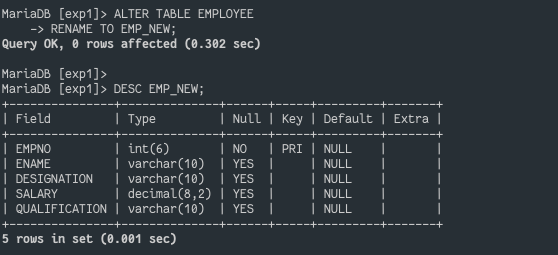
\includegraphics{img/p1/ss4.png}
			\begin{verbatim}
				ALTER TABLE EMP\_NEW
				DROP COLUMN QUALIFICATION;

				DESC EMP_NEW;
			\end{verbatim}
			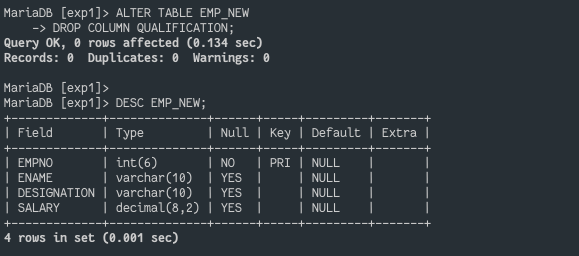
\includegraphics{img/p1/ss5.png}
		
		\item Truncate the table EMP\_NEW \\
		Syntax: 
		\begin{verbatim}
			INSERT INTO EMP_NEW 
			VALUES (1, "Name1", "Manager", 2000.00);

			SELECT * FROM EMP_NEW;

			TRUNCATE TABLE EMPLOYEE;

			SELECT * FROM EMP_NEW;
		\end{verbatim}
		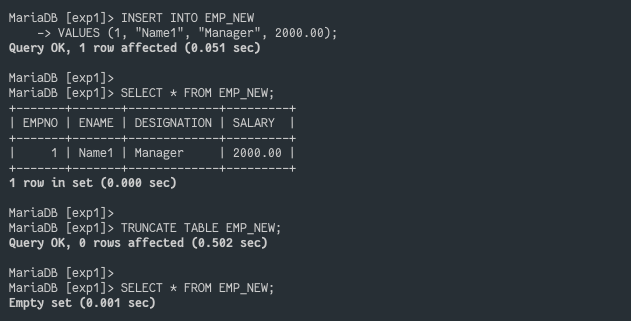
\includegraphics{img/p1/ss6.png}

		\item Drop the table \\
		Syntax: 
		\begin{verbatim}
			DROP TABLE EMP_NEW;

			DESC EMP_NEW;
		\end{verbatim}
		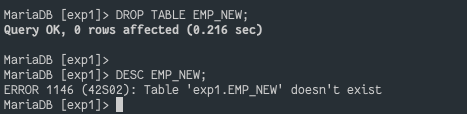
\includegraphics{img/p1/ss7.png}
	\end{enumerate}

	\section*{Result}
	Implemented the program for creating and modifying a table using MariaDB 10.5 and the following output
	were obtained.

	\newpage

	\begin{frame}{}
		\centering
		\hspace*{-0.5cm}
		$\vcenter{\hbox{
\includegraphics[width=1.5cm]{img/emblem.jpeg}}}$
		$\vcenter{\resizebox{0.95\textwidth}{!}{
			\begin{tabular}{c}
				 CS333 - Application Software Development Lab $\cdot$ 2020 $\cdot$   \\
				 \hline 
			\end{tabular}
		}}$
	\end{frame}
	\section*{Cycle 1}
	\section*{Expt 2}
	\begin{center}
		\Large{Basic SQL Queries - I}
	\end{center}
	
	\section*{Aim}
	\large{To study the basic queries such as
		\begin{enumerate}
			\item SELECT
			\item INSERT
			\item UPDATE
			\item DELETE
		\end{enumerate}
	}
	
	\section*{Experiment}
		\begin{enumerate}
			\item 
				Insert records into the employee table (Fields : EmpId, Ename,
	Designation, Salary, Dept.id) created.
				
				 Synatx:
				\begin{verbatim}
	CREATE TABLE Employee(
		Emp_no INT(6) PRIMARY KEY,
		Ename VARCHAR(10),
		Designation VARCHAR(10),
		Salary INT(6),
		Dept_id INT(4)
	);
	
	INSERT INTO Employee
	VALUES
		(66928, "BLAZE", "MANAGER", 55000, 3001),
		(67832, "CLARE", "MANAGER", 51000, 1001),
		(65646, "JONAS", "MANAGER", 59140, 2001),
		(67858, "SCARLET", "ANALYST", 62000, 2001),
		(69062, "FRANK", "ANALYST", 62000, 2001),
		(63679, "SANDRINE", "CLERK", 18000, 3001),
		(64989, "ADELYN", "SALESMAN", 34000, 3001),
		(65271, "WADE", "SALESMAN", 27000, 3001),
		(66564, "MADDEN", "SALESMAN", 27000, 3001),
		(68454, "TUCKER", "SALESMAN", 32000, 3001),
		(68736, "ANDRES", "CLERK", 24000, 2001),
		(69000, "JULIUS", "CLERK", 21000, 3001),
		(69324, "MARKER", "CLERK", 28000, 1001);
				\end{verbatim}
				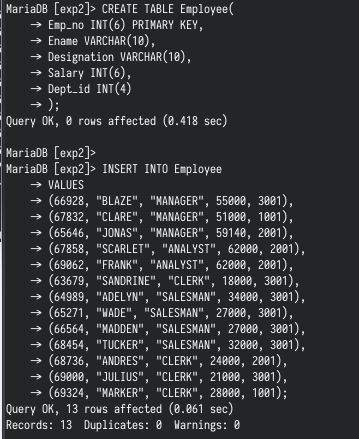
\includegraphics{img/p2/ss1.png}
			
				\item 
				Display the details of all the employees.
				
				Syntax:
				\begin{verbatim}
	SELECT * FROM Employee;
				\end{verbatim}
				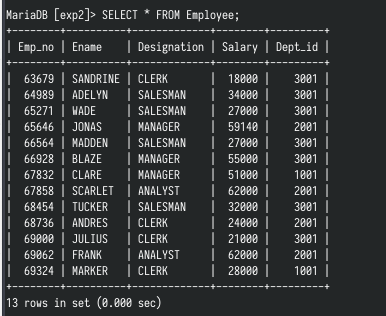
\includegraphics{img/p2/ss2.png}
			
			\item 
			Display the employee numbers, names and designation of all employees.
			
			Syntax:
			\begin{verbatim}
	SELECT Emp_no, Ename, Designation
	FROM Employee;
			\end{verbatim}
			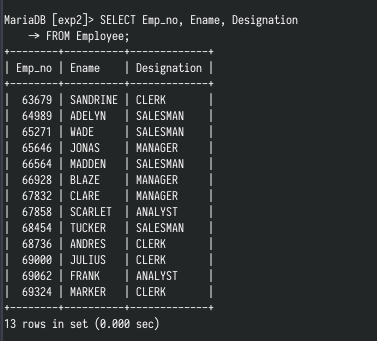
\includegraphics{img/p2/ss3.png}
	
			\item
			Suppose the emp\_no 68454 has left the company. Delete the employee
	from the database.
			Syntax: 
			\begin{verbatim}
	DELETE FROM Employee
	WHERE Emp_no=68454;
			\end{verbatim}
		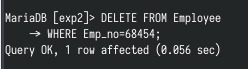
\includegraphics{img/p2/ss4.png}
		
		\item
		Suppose a new employee joins the company under department 2001 as
	an analyst. The salary of the employee is not yet fixed. Add his record to
	the database.
	
		Syntax:
		\begin{verbatim}
	INSERT INTO Employee
	(Emp_no, Ename, Designation, Dept_id) VALUES
		(69876, "Rahul", "ANALYST", 2001);
		\end{verbatim}
		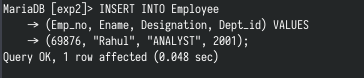
\includegraphics[]{img/p2/ss5.png}
		5.jp
	\item
	Find the details of employees with salary > 25000 working in department
	with id 2001.
	
	Syntax:
	\begin{verbatim}
	SELECT * FROM Employee
	WHERE Salary>25000 AND Dept_id=2001;
	\end{verbatim}
	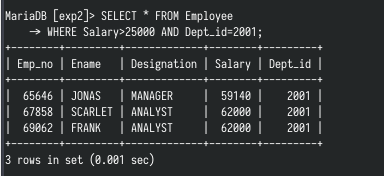
\includegraphics[]{img/p2/ss6.png}
	
	\item
			Suppose the newly added employee's salary is now fixed. Add his salary
	details.
			Syntax: 
			\begin{verbatim}
	UPDATE Employee
	SET Salary=40000
	WHERE Emp_no=69876;
			\end{verbatim}
			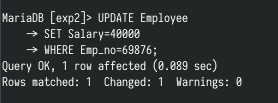
\includegraphics{img/p2/ss7.png}
			
		\item
		Suppose the employee ADELYN is now promoted as Analyst. Update his
	designation and salary.
	Syntax:
		\begin{verbatim}
	UPDATE Employee
	SET Designation="ANALYST", Salary=40000
	WHERE Ename="ADELYN";
		\end{verbatim}
		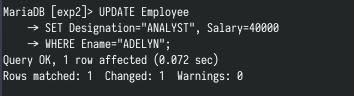
\includegraphics[]{img/p2/ss8.png}
		
		\item
		Display the names of all managers and analysts.
	Syntax:
		\begin{verbatim}
	SELECT * FROM Employee
	WHERE Designation="MANAGER" OR Designation="ANALYST";
		\end{verbatim}
		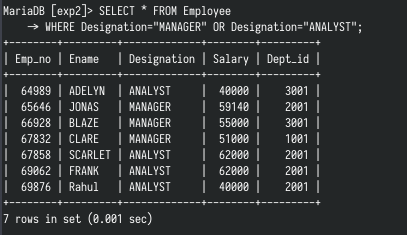
\includegraphics[]{img/p2/ss9.png}
		
			\item
	Retrieve the names of all employees whose salary is between 30000
	and 60000.
		\begin{verbatim}
	SELECT * FROM Employee
	WHERE Salary>30000 AND Salary<60000;
		\end{verbatim}
		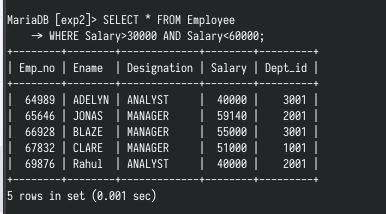
\includegraphics[]{img/p2/ss10.png}
		
			\item
	A salary hike is now announced by dept. 2001. Update the salary of all
	their employees by 5\%.
	
		\begin{verbatim}
	UPDATE Employee
	SET Salary = Salary + Salary*(0.05)
	WHERE Dept_id=2001;
		\end{verbatim}
		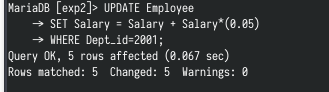
\includegraphics[]{img/p2/ss11.png}
		
				\item
	List all employees whose salary is less than 30000 or working for dept.
	1001.
	
		\begin{verbatim}
	SELECT * FROM Employee
	WHERE Salary<30000 OR Dept_id=1001;
	
		\end{verbatim}
		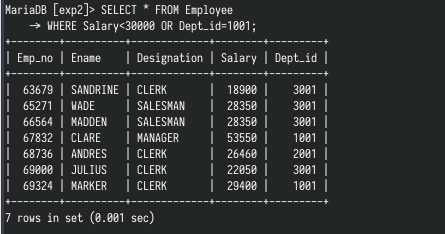
\includegraphics[]{img/p2/ss12.png}
		
		\end{enumerate}
		\section*{Result}
		Implemented the program for basic sql queries using MariaDB 10.5 and the following output
	were obtained.

		\newpage

		\begin{frame}{}
			\centering
			\hspace*{-0.5cm}
			$\vcenter{\hbox{
\includegraphics[width=1.5cm]{img/emblem.jpeg}}}$
			$\vcenter{\resizebox{0.95\textwidth}{!}{
				\begin{tabular}{c}
					 CS333 - Application Software Development Lab $\cdot$ 2020 $\cdot$   \\
					 \hline 
				\end{tabular}
			}}$
		\end{frame}
		\section*{Cycle 1}
		\section*{Expt 3}
		\begin{center}
			\Large{Basic SQL Queries - II}
		\end{center}
		
		\section*{Aim}
		\large{Understand basic SQL queries
		\begin{enumerate}
			\item ALTER
			\item RENAME
			\item SELECT DISTINCT
			\item SQL IN
			\item SQL BETWEEN
			\item SQL ALIASES
			\item SQL AND
			\item SQL OR
		\end{enumerate}
		}
		\section*{Experiment}
			\begin{enumerate}
		\item
		Create a CAR database with the following details.
		\begin{verbatim}
		
			+----+--------+------------+---------+-------------+
			| id | name   | company    | country | approxprice |
			+----+--------+------------+---------+-------------+
			|  1 | Beat   | Chevrolet  | USA     |         4.0 |
			|  2 | Swift  | Maruti     | Japan   |         6.0 |
			|  3 | Escort | Ford       | USA     |         4.2 |
			|  4 | Sunny  | Nissan     | Japan   |         8.0 |
			|  5 | Beetle | Volkswagen | Germany |        21.0 |
			|  6 | Etios  | Toyota     | Japan   |         7.2 |
			|  7 | Sail   | Chevrolet  | USA     |         5.0 |
			|  8 | Aria   | Tata       | India   |         7.0 |
			|  9 | Passat | Volkswagen | Germany |        25.0 |
			| 10 | SX4    | Maruti     | Japan   |         6.7 |
			+----+--------+------------+---------+-------------+
		\end{verbatim}
		 
		Syntax:
		\begin{verbatim}
		CREATE TABLE CAR(
				id INT PRIMARY KEY,
				name VARCHAR(10),
				company VARCHAR(20),
				country VARCHAR(10),
				approxprice DECIMAL(1, 3)
		);
		INSERT INTO CAR 
		VALUES
				(1, 'Beat', 'Chevrolet', 'USA', 4),
				(2, 'Swift', 'Maruti', 'Japan', 6),
				(3, 'Escort', 'Ford', 'USA', 4.2),
				(4, 'Sunny', 'Nissan', 'Japan', 8),
				(5, 'Beetle', 'Volkswagen', 'Germany', 21),
				(6, 'Etios', 'Toyota', 'Japan', 7.2),
				(7, 'Sail', 'Chevrolet', 'USA', 5),
				(8, 'Aria', 'Tata', 'India', 7),
				(9, 'Passat', 'Volkswagen', 'Germany', 25),
				(10, 'SX4', 'Maruti', 'Japan', 6.7);
		
		\end{verbatim}
		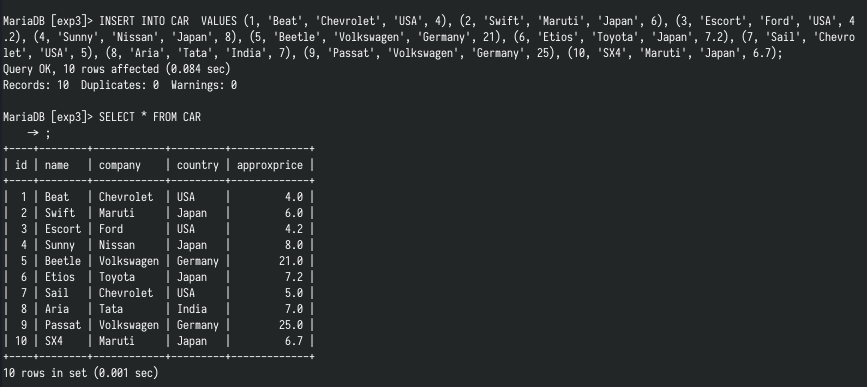
\includegraphics[width=\textwidth]{img/p3/ss1.png}
		
		
		\item
		List the car companies in the database.
		 
		Syntax:
		\begin{verbatim}
		SELECT company 
		FROM CAR;
		
		\end{verbatim}
		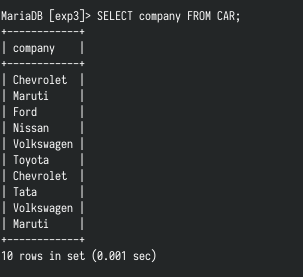
\includegraphics[]{img/p3/ss2.png}
		
		
		\item
		List the names of countries with car production companies.
		 
		Syntax:
		\begin{verbatim}
		SELECT country 
		FROM CAR;
		
		\end{verbatim}
		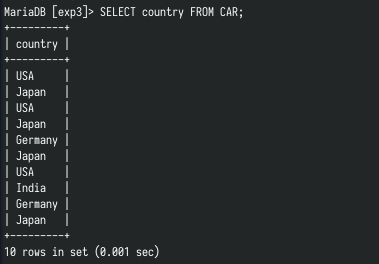
\includegraphics[]{img/p3/ss3.png}
		
		
		\item
		List the details of cars within a price range 4 to 7 lakhs.
		 
		Syntax:
		\begin{verbatim}
		SELECT *
		FROM CAR
		WHERE approxprice>4 AND approxprice<7;
		
		\end{verbatim}
		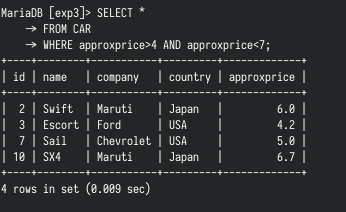
\includegraphics[]{img/p3/ss4.png}
		
		
		\item
		List the name and company of all the cars originating from India and
		 having price <= 8 lakhs.
		 
		Syntax:
		\begin{verbatim}
		SELECT name, company
		FROM CAR
		WHERE country='India' AND approxprice<=8;
		
		\end{verbatim}
		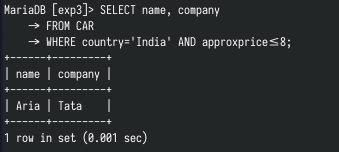
\includegraphics[]{img/p3/ss5.png}
		
		
		\item
		List the names, companies and countries of cars either from Nissan or
		 from Germany.
		 
		Syntax:
		\begin{verbatim}
		SELECT name, company, country
		FROM CAR
		where company='Nissan' OR country='Germany';
		
		\end{verbatim}
		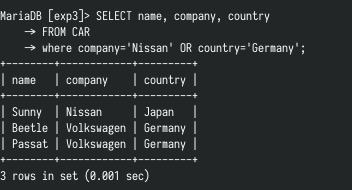
\includegraphics[]{img/p3/ss6.png}
		
		
		\item
		List the names of all cars produced by (Maruti,Ford). Use SQL IN
		 statement.
		 
		Syntax:
		\begin{verbatim}
		SELECT name
		FROM CAR
		WHERE company IN ('Maruti', 'Ford');
		
		\end{verbatim}
		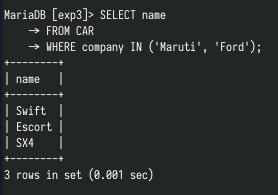
\includegraphics[]{img/p3/ss7.png}
		
		
		\item
		Alter the table cars to add a new field year (model release year). Update
		 the year column for all the rows in the database.
		 
		Syntax:
		\begin{verbatim}
		ALTER TABLE CAR
		ADD COLUMN year INT;
		UPDATE CAR
		SET year=2010;
		
		\end{verbatim}
		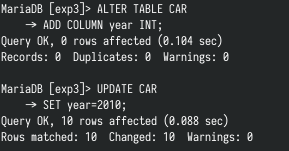
\includegraphics[]{img/p3/ss8.png}
		
		
		\item
		Retrieve the names of all cars and display names under 'Car\_name'.
		 
		Syntax:
		\begin{verbatim}
		SELECT name AS 'Car_name'
		FROM CAR
		
		\end{verbatim}
		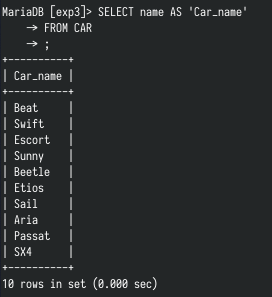
\includegraphics[]{img/p3/ss9.png}
		
		
		\item
		Rename the attribute name to car\_name.
		 
		Syntax:
		\begin{verbatim}
		ALTER TABLE CAR
		CHANGE COLUMN name Car_name VARCHAR(10);
		
		\end{verbatim}
		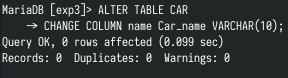
\includegraphics[]{img/p3/ss10.png}
		
		
		\item
		List the car manufactured by Toyota (to be displayed as cars\_Toyota).
		 
		Syntax:
		\begin{verbatim}
		SELECT Car_name AS 'cars_Toyota'
		FROM CAR
		WHERE company='Toyota';
		
		\end{verbatim}
		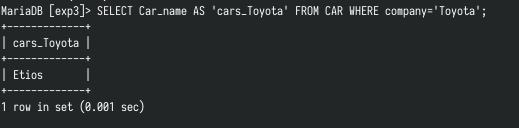
\includegraphics[]{img/p3/ss11.png}
		
		
		\item
		List the details of all cars in alphabetical order.
		 
		Syntax:
		\begin{verbatim}
		SELECT *
		FROM CAR
		ORDER BY Car_name ASC;
		
		\end{verbatim}
		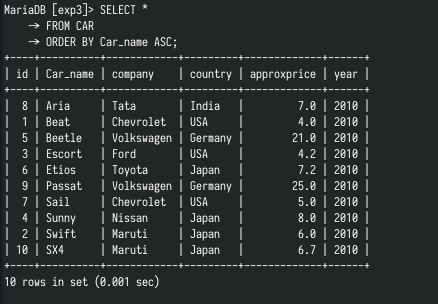
\includegraphics[]{img/p3/ss12.png}
		
		
		\item
		List the details of all cars from cheapest to costliest.
		
		Syntax:
		\begin{verbatim}
		SELECT *
		FROM CAR
		ORDER BY approxprice ASC;
		
		\end{verbatim}
		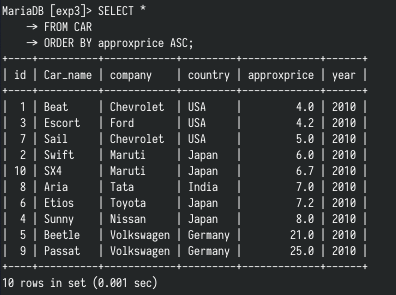
\includegraphics[]{img/p3/ss13.png}
			\end{enumerate}
			\section*{Result}
			Implemented the program for various select options using MariaDB 10.5 and the following output
	were obtained.

			\newpage

			\begin{frame}{}
				\centering
				\hspace*{-0.5cm}
				$\vcenter{\hbox{
\includegraphics[width=1.5cm]{img/emblem.jpeg}}}$
				$\vcenter{\resizebox{0.95\textwidth}{!}{
					\begin{tabular}{c}
						 CS333 - Application Software Development Lab $\cdot$ 2020 $\cdot$   \\
						 \hline 
					\end{tabular}
				}}$
			\end{frame}
			\section*{Cycle 1}
			\section*{Expt 4}
			\begin{center}
				\Large{Introduction to Aggregate functions}
			\end{center}
			
			\section*{Aim}
			\large{Introduction to Aggregate functions
			\begin{enumerate}
				\item AVG
				\item MIN
				\item MAX
				\item SUM
				\item COUNT
			\end{enumerate}
			}

			\section*{Theory}
			Sum( fieldname) Returns the total sum of the field.\\
• Avg(fieldname) Returns the average of the field.\\
• Count( ) Count function has three variations:\\
• Count(*) : returns the number of rows in the table including duplicates and
those with null values\\
• Count(fieldname) : returns the number of rows where field value is not null\\
Count (All): returns the total number of rows. It is same like count(*)\\
• Max(fieldname) Returns the maximum value of the field\\
• Min(fieldname) Returns the maximum value of the field\\
			
			\section*{Experiment}
				\begin{enumerate}
					\item
					Create a table named Student and populate the table. 
							a. The table contains the marks of 10 students for 3 subjects(Physics, Chemistry, 
					 Mathematics). 
							b. The total marks for physics and chemistry is 25, while for mathematics it is 50. 
							c. The pass mark for physics and chemistry is 12 and for mathematics it is 25. 
							d. A student is awarded a ‘Pass’ if he has passed all the subjects.
					\begin{verbatim}
						+----------+----------+---------+-----------+-------------+
						| roll_num | name     | physics | chemistry | mathematics |
						+----------+----------+---------+-----------+-------------+
						|        1 | Adam     |      20 |        20 |          33 |
						|        2 | Bob      |      18 |         9 |          41 |
						|        3 | Bright   |      22 |         7 |          31 |
						|        4 | Duke     |      13 |        21 |          20 |
						|        5 | Elvin    |      14 |        22 |          23 |
						|        6 | Fetcher  |       2 |        10 |          48 |
						|        7 | Georgina |      22 |        12 |          22 |
						|        8 | Mary     |      24 |        14 |          31 |
						|        9 | Tom      |      19 |        15 |          24 |
						|       10 | Zack     |       8 |        20 |          36 |
						+----------+----------+---------+-----------+-------------+
					\end{verbatim}
					 
					Syntax:
					\begin{verbatim}
					CREATE TABLE IF NOT EXISTS Student (
							roll_num INT PRIMARY KEY,
							name VARCHAR(10),
							physics INT,
							chemistry INT,
							mathematics INT
					);
					INSERT INTO Student 
					VALUES
							(1, "Adam", 20, 20, 33), 
							(2, "Bob", 18, 9, 41), 
							(3, "Bright", 22, 7, 31),
							(4, "Duke", 13, 21, 20),
							(5, "Elvin", 14, 22, 23),
							(6, "Fetcher", 2, 10, 48),
							(7, "Georgina", 22, 12, 22), 
							(8, "Mary", 24, 14, 31),
							(9, "Tom", 19, 15, 24),
							(10, "Zack", 8, 20, 36);
					SELECT * FROM Student;
					
					\end{verbatim}
					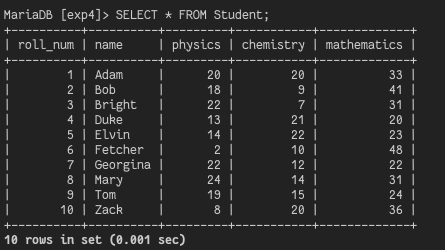
\includegraphics[]{img/p4/ss1.png}
					
					
					\item
					Find the class average for the subject ‘Physics’ 
					 
					Syntax:
					\begin{verbatim}
					SELECT AVG(physics)
					FROM Student;
					
					\end{verbatim}
					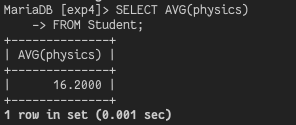
\includegraphics[]{img/p4/ss2.png}
					
					
					\item
					Find the highest marks for mathematics (To be displayed as highest\_marks\_maths). 
					 
					Syntax:
					\begin{verbatim}
					SELECT MAX(mathematics) as 'highest_marks_maths'
					FROM Student;
					
					\end{verbatim}
					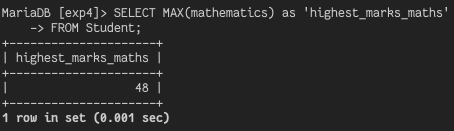
\includegraphics[]{img/p4/ss3.png}
					
					
					\item
					Find the lowest marks for chemistry(To be displayed as lowest\_mark\_chemistry) 
					 
					Syntax:
					\begin{verbatim}
					SELECT MIN(chemistry) as 'lowest_mark_chemistry'
					FROM Student;
					
					\end{verbatim}
					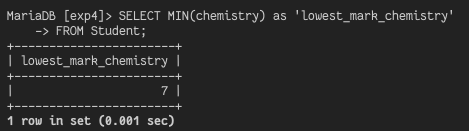
\includegraphics[]{img/p4/ss4.png}
					
					
					\item
					Find the total number of students who has got a pass in physics
					 
					Syntax:
					\begin{verbatim}
					SELECT COUNT(*)
					FROM Student
					WHERE physics >= 12;
					
					\end{verbatim}
					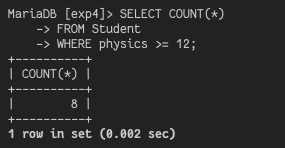
\includegraphics[]{img/p4/ss5.png}
					
					
					\item
					Generate the list of students who have passed in all the subjects. 
					 
					Syntax:
					\begin{verbatim}
					SELECT *
					FROM Student
					WHERE physics >= 12 AND chemistry >= 12 AND mathematics >= 25;
					
					\end{verbatim}
					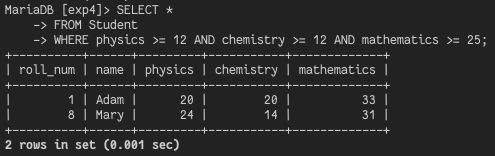
\includegraphics[]{img/p4/ss6.png}
					
					
					\item
					Generate a rank list for the class. Indicate Pass/Fail. 
					 
					Syntax:
					\begin{verbatim}
					ALTER TABLE Student
					ADD COLUMN Status VARCHAR(4) DEFAULT 'Fail';
					UPDATE Student
					SET Status='Pass'
					WHERE physics >= 12 AND chemistry >= 12 AND mathematics >= 25;
					SELECT *
					FROM Student
					ORDER BY (physics+chemistry+mathematics);
					
					\end{verbatim}
					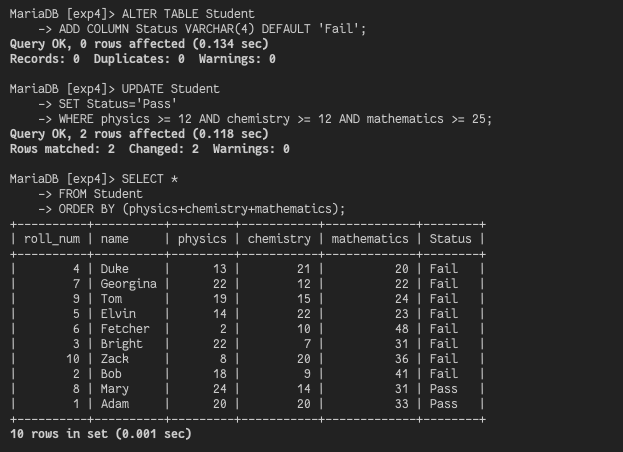
\includegraphics[width=\textwidth]{img/p4/ss7.png}
					
					
					\item
					Find pass percentage of the class for mathematics. 
					 
					Syntax:
					\begin{verbatim}
					SELECT 100*COUNT(*)/(SELECT COUNT(*) FROM Student) as 'math_pass_percentage'
					FROM Student
					WHERE mathematics >= 25;
					
					\end{verbatim}
					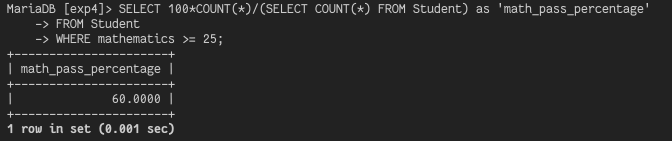
\includegraphics[width=\textwidth]{img/p4/ss8.png}
					
					
					\item
					Find the overall pass percentage for all class. 
					 
					Syntax:
					\begin{verbatim}
					SELECT 100*COUNT(*)/(SELECT COUNT(*) FROM Student) as 'pass_percentage'
					FROM Student
					WHERE Status='Pass';
					
					\end{verbatim}
					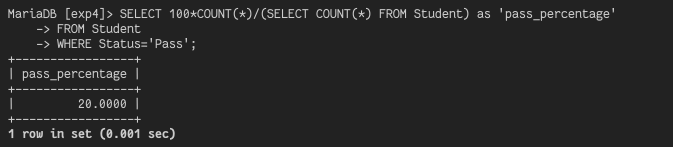
\includegraphics[width=\textwidth]{img/p4/ss9.png}
					
					
					\item
					Find the class average. 
					 
					Syntax:
					\begin{verbatim}
					SELECT AVG(physics+chemistry+mathematics)
					FROM Student;
					
					\end{verbatim}
					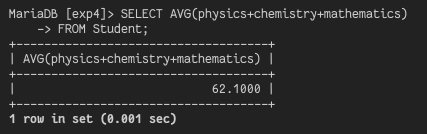
\includegraphics[]{img/p4/ss10.png}
					
					
					\item
					Find the total number of students who have got a Pass.
					
					Syntax:
					\begin{verbatim}
					SELECT COUNT(*) as 'passed'
					FROM Student
					WHERE Status='Pass';
					\end{verbatim}
					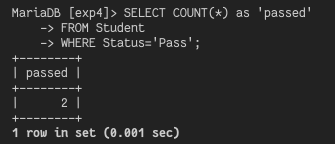
\includegraphics[]{img/p4/ss11.png}
				\end{enumerate}		
				\section*{Result}
				Implemented the program for various aggregate functions using MariaDB 10.5 and the following output
	were obtained.

				\newpage

				\begin{frame}{}
					\centering
					\hspace*{-0.5cm}
					$\vcenter{\hbox{
\includegraphics[width=1.5cm]{img/emblem.jpeg}}}$
					$\vcenter{\resizebox{0.95\textwidth}{!}{
						\begin{tabular}{c}
							 CS333 - Application Software Development Lab $\cdot$ 2020 $\cdot$   \\
							 \hline 
						\end{tabular}
					}}$
				\end{frame}
				\section*{Cycle 1}
				\section*{Expt 5}
				\begin{center}
					\Large{Data Constraint and Views}
				\end{center}
				
				\section*{Aim}
				\large To study about various data constraints and views in SQL.
				\section*{Theory}
				\textbf{SQL Constraints}
SQL constraints are used to specify rules for the data in a table.
Constraints are used to limit the type of data that can go into a table. This ensures
the accuracy and reliability of the data in the table. If there is any violation between
the constraint and the data action, the action is aborted.
Constraints can be column level or table level. Column level constraints apply to a
column, and table level constraints apply to the whole table. The following constraints
are commonly used in SQL:\\
• NOT NULL - Ensures that a column cannot have a NULL value\\
• UNIQUE - Ensures that all values in a column are different\\
• PRIMARY KEY - A combination of a NOT NULL and UNIQUE. Uniquely identifies each row in a table\\
• FOREIGN KEY - Uniquely identifies a row/record in another table\\
• CHECK - Ensures that all values in a column satisfies a specific condition\\
• DEFAULT - Sets a default value for a column when no value is specified\\
• INDEX - Used to create and retrieve data from the database very quickly\\
\textbf{SQL CREATE VIEW Statement}
In SQL, a view is a virtual table based on the result-set of an SQL statement.
A view contains rows and columns, just like a real table. The fields in a view are
fields from one or more real tables in the database.
You can add SQL functions, WHERE, and JOIN statements to a view and present
the data as if the data were coming from one single table.
				\section*{Expiriment}
				\begin{itemize}
					\item
					\begin{verbatim}
					Create the following tables with given constraints. 
							a. Create a table named Subjects with the given attributes. 
									• Sub_id ( Should not be NULL) 
									• Sub_name (Should not be NULL) 
									• Populate the database. Make sure that all constraints are working properly. 
									Sub_id Sub_name 
									1 Maths 
									2 Physics 
									3 Chemistry 
									4 English 
									i. Alter the table to set Sub_id as the primary key. 
							b. Create a table named Staff with the given attributes. 
									• Staff_id (Should be UNIQUE) 
									• Staff_name 
									• Dept 
									• Age ( Greater than 22) 
									• Salary (Less than 35000) 
									Staff_id Staff_name Dept Age Salary 
									1 John Purchasing 24 30000 
									2 Sera Sales 25 20000 
									3 Jane Sales 28 25000 
									i. Delete the check constraint imposed on the attribute Salary. 
									ii. Delete the unique constraint on the attribute Staff_id. 
							c. Create a table named Bank with the following attributes. 
									• Bank_code (To be set as Primary Key, type= varchar(3) ) 
									• Bank_name (Should not be NULL) 
									• Head_office 
									• Branches (Integer value greater than Zero) 
									i. Make sure that all constraints are working properly. All constraints 
									have to be set after creating the table. 
									Bank_code Bank_name Head_office Branches 
									AAA SIB Ernakulam 6 
									BBB Federal Kottayam 5 
									CCC Canara Trivandrum 3 
									SBT Indian Delhi 7 
							d. Create a table named Branch with the following attributes. 
									• Branch_id (To be set as Primary Key) 
									• Branch_name (Set Default value as ‘New Delhi") 
									• Bank_id (Foreign Key:- Refers to bank code of Bank table) 
									i. Populate the database. Make sure that all constraints are working 
									properly. 
									Branch_id Branch_name Bank_id 
									1 Kottayam CCC 5 Calicut SBT 
									ii. During database population, demonstrate how the DEFAULT 
									Constraint is satisfied. (Insert values with branch as “New Delhi”)
									 iii. Delete the bank with 
									bank code "SBT" and make sure that the 
									corresponding entries are getting deleted from the related tables. 
									iv. Drop the Primary Key using ALTER command 
					\end{verbatim}
				Syntax: 	
				\begin{verbatim}
					CREATE TABLE IF NOT EXISTS Subjects (
							Sub_id INT NOT NULL,
							Sub_name VARCHAR(10) NOT NULL
					);
					INSERT INTO Subjects
					VALUES
							(1, "Maths"),
							(2, "Physics"),
							(3, "Chemistry"),
							(4, "English");
					ALTER TABLE Subjects
					ADD PRIMARY KEY(Sub_id);
					CREATE TABLE IF NOT EXISTS Staff (
							Staff_id INT NOT NULL UNIQUE,
							Staff_name VARCHAR(10),
							Dept VARCHAR(10),
							Age INT,
							Salary INT,
							CHECK(AGE > 22), 
							CONSTRAINT Staff_Staff_id_key UNIQUE Staff_id,
							CONSTRAINT Staff_Salary_check CHECK(Salary < 35000)
					);
					INSERT Into Staff
					VALUES
							("1","John","Purchasing","24","30000"),
							("2","Sera","Sales","25","20000"),
							("3","Jane","Sales","28","25000");
					ALTER TABLE Staff
					DROP CONSTRAINT Staff_Salary_check;
					ALTER TABLE Staff
					DROP CONSTRAINT Staff_Staff_id_key;
					CREATE TABLE IF NOT EXISTS Bank (
							Bank_code VARCHAR(3),
							Bank_name VARCHAR(10),
							Head_office VARCHAR(10),
							Branches INT
					);
					ALTER TABLE Bank
					ADD CONSTRAINT primary_key PRIMARY KEY (Bank_code);
					ALTER TABLE Bank
					ADD CONSTRAINT branch_office CHECK (Branches > 0);
					INSERT INTO Bank
					VALUES
							("AAA", "SIB", "Ernakulam", 6),
							("BBB", "Federal", "Kottayam", 5),
							("CCC", "Canara", "Trivandrum", 3);
					CREATE TABLE IF NOT EXISTS Branch (
							Branch_id INT,
							Branch_name VARCHAR(10) DEFAULT 'New Delhi',
							Bank_id VARCHAR(3),
							CONSTRAINT Branch_pkey PRIMARY KEY (Branch_id) 
					);
					ALTER TABLE Branch
					ADD CONSTRAINT Branch_Bank_id_fkey 
							FOREIGN KEY (Bank_id) REFERENCES Bank(Bank_code) ON UPDATE CASCADE ON DELETE CASCADE;
					INSERT INTO Branch
					VALUES
							(1, "Kottayam", "CCC"),
							(2, NULL, "AAA");
					INSERT INTO Bank
					VALUES ("SBT", "Indian", "Delhi", 7);
					INSERT INTO Branch
					VALUES (5, "Calicut", "SBT");
					DELETE FROM Bank
					WHERE Bank_code='SBT';
					ALTER TABLE Branch
					DROP CONSTRAINT Branch_pkey;
					INSERT INTO Branch
					VALUES (1, "PPP", "CCC");
					
					\end{verbatim}
					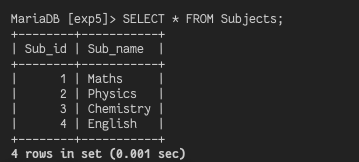
\includegraphics[]{img/p5/ss1.1.png} \\
					\includegraphics[]{img/p5/ss1.2.png} \\
					\includegraphics[]{img/p5/ss1.3.png} \\
					\includegraphics[]{img/p5/ss1.4.png} \\
					\includegraphics[]{img/p5/ss1.5.png} \\
					\includegraphics[]{img/p5/ss1.6.png} \\
					
					
					\item
					Create a View named sales\_staff to hold the details of all staff working in sales 
							Department. (Refer to table Staff in question 1(b)) 
					 
					Syntax:
					\begin{verbatim}
					CREATE VIEW sales_staff AS 
							(SELECT * FROM Staff WHERE Dept="SALES");
					SELECT * FROM sales_staff;
					
					\end{verbatim}
					\includegraphics[]{img/p5/ss2.png}
					
					
					\item
					Drop table branch. Create another table named branch and name all the constraints as 
							given below: 
							• Constraint name Column Constraint 
							• Pk branch\_id Primary key 
							• Df branch\_name Default :"New Delhi" 
							• Fk bankid Foreign key/References 
							i. Delete the default constraint in the table ii. Delete the primary key constraint 
					 
					Syntax:
					\begin{verbatim}
					DROP TABLE Branch;
					CREATE TABLE Branch (
							Branch_id INT,
							Branch_name VARCHAR(10) CONSTRAINT Df DEFAULT 'New Delhi',
							Bank_id VARCHAR(3),
							CONSTRAINT Pk PRIMARY KEY (Branch_id),
							CONSTRAINT Fk FOREIGN KEY (Bank_id) REFERENCES Bank (Bank_code) ON UPDATE CASCADE ON DELETE CASCADE
					);
					ALTER TABLE Branch 
					DROP CONSTRAINT Df;
					ALTER TABLE Branch
					DROP CONSTRAINT Pk;
					
					\end{verbatim}
					
					
					\item
					Update the view sales staff to include the details of staff belonging to sales department whose salary is greater than 20000. 
					 
					Syntax:
					\begin{verbatim}
					CREATE OR REPLACE VIEW sales_staff 
					AS (SELECT * FROM Staff WHERE Salary > 20000 AND Dept="Sales");
					
					\end{verbatim}
					\includegraphics[]{img/p5/ss4.png}
					
					
					\item
					Delete the view sales staff.
					
					Syntax:
					\begin{verbatim}
					DROP VIEW sales_staff;
					\end{verbatim}
					\includegraphics[]{img/p5/ss5.png}
				\end{itemize}
				\section*{Result}
				Implemented the program for data constraints and views using MariaDB 10.5 and the following output
				were obtained.
					\newpage

					\begin{frame}{}
						\centering
						\hspace*{-0.5cm}
						$\vcenter{\hbox{\includegraphics[width=1.5cm]{img/emblem.jpeg}}}$
						$\vcenter{\resizebox{0.95\textwidth}{!}{
							\begin{tabular}{c}
								 CS333 - Application Software Development Lab $\cdot$ 2020 $\cdot$   \\
								 \hline 
							\end{tabular}
						}}$
					\end{frame}
					\section*{Cycle 1}
					\section*{Expt 6}
					\begin{center}
						\Large{String Functions and Pattern Matching}
					\end{center}
					
					\section*{Aim}
					\large To study about String Functions \& Pattern Matching.
					\section*{Theory}
					ASCII	Return the ASCII code value of a character
CHAR	Convert an ASCII value to a character\\
CHARINDEX	Search for a substring inside a string starting from a specified location and return the position of the substring.\\
CONCAT	Join two or more strings into one string\\
CONCAT\_WS	Concatenate multiple strings with a separator into a single string\\
DIFFERENCE	Compare the SOUNDEX() values of two strings\\
FORMAT	Return a value formatted with the specified format and optional culture\\
LEFT	Extract a given a number of characters from a character string starting from the left\\
LEN	Return a number of characters of a character string\\
LOWER	Convert a string to lowercase\\
LTRIM	Return a new string from a specified string after removing all leading blanks\\
NCHAR	Return the Unicode character with the specified integer code, as defined by the Unicode standard\\
PATINDEX	Returns the starting position of the first occurrence of a pattern in a string.\\
QUOTENAME	Returns a Unicode string with the delimiters added to make the input string a valid delimited identifier\\
REPLACE	Replace all occurrences of a substring, within a string, with another substring\\
REPLICATE	Return a string repeated a specified number of times\\
REVERSE	Return the reverse order of a character string\\
RIGHT	Extract a given a number of characters from a character string starting from the right\\
RTRIM	Return a new string from a specified string after removing all trailing blanks\\
SOUNDEX	Return a four-character (SOUNDEX) code of a string based on how it is spoken\\
SPACE	Returns a string of repeated spaces.\\
STR	Returns character data converted from numeric data.\\
STRING\_AGG	Concatenate rows of strings with a specified separator into a new string\\
STRING\_ESCAPE	Escapes special characters in a string and returns a new string with escaped characters\\
STRING\_SPLIT	A table-valued function that splits a string into rows of substrings based on a specified separator.\\
STUFF	Delete a part of a string and then insert another substring into the string starting at a specified position.\\
SUBSTRING	Extract a substring within a string starting from a specified location with a specified length\\
TRANSLATE	Replace several single-characters, one-to-one translation in one operation.\\
TRIM	Return a new string from a specified string after removing all leading and trailing blanks\\
UNICODE	Returns the integer value, as defined by the Unicode standard, of a character.\\
UPPER	Convert a string to uppercase
					\section*{Expiriment}
					\begin{itemize}
					\item 
					Syntax:
					\begin{verbatim}
						CREATE TABLE acct_details (
						acct_no CHAR(9) PRIMARY KEY,
						branch VARCHAR(10),
						name VARCHAR(30),
						phone VARCHAR(15)	
					);
						INSERT INTO acct_details 
					VALUES ('A40123401','Chicago' ,'Mike Adams' ,'(378)400-1234'),
						('A40123402','Miami','Diana George','(372)420-2345'),
						('B40123403','Miami','Diaz Elizabeth','(371)450-3456'),
						('B40123404','Atlanta','Jeoffrey George','(370)460-4567'),
						('B40123405','New York','Jennifer Kaitlyn','(373)470-5678'),
						('C40123406','Chicago','Kaitlyn Vincent','(318)200-3235'),
						('C40123407','Miami','Abraham Gottfield','(328)300-2256'),
						('C50123408','New Jersey','Stacy Williams','(338)400-5237'),
						('D50123409','New York','Catherine George','(348)500-6228'),
						('D50123410','Miami','Oliver Scott','(358)600-7230');
					SELECT * FROM acct_details;
					\end{verbatim}
					\includegraphics[]{img/p6/ss0.png}
					
					\item
					Find the names of all people starting on the alphabet 'D’.
					 
					Syntax:
					\begin{verbatim}
					SELECT name FROM acct_details
					WHERE name LIKE 'D%';
					
					\end{verbatim}
					\includegraphics[]{img/p6/ss1.png}
					
					
					\item
					List the names of all branches containing the substring 'New’
					 
					Syntax:
					\begin{verbatim}
					SELECT branch FROM acct_details
					WHERE branch LIKE '%New%';
					
					\end{verbatim}
					\includegraphics[]{img/p6/ss2.png}
					
					
					\item
					List all the names in Upper Case Format
					 
					Syntax:
					\begin{verbatim}
					SELECT UPPER(name) FROM acct_details;
					
					\end{verbatim}
					\includegraphics[]{img/p6/ss3.png}
					
					
					\item
					List the names where the 4th letter is 'n’ and last letter is 'n’
					 
					Syntax:
					\begin{verbatim}
					SELECT name FROM acct_details
					WHERE name LIKE '___n%n';
					
					\end{verbatim}
					\includegraphics[]{img/p6/ss4.png}
					
					
					\item
					List the names starting on 'D’, 3rd letter is 'a’ and contains the substring 'Eli’
					 
					Syntax:
					\begin{verbatim}
					SELECT name FROM acct_details
					WHERE name LIKE 'D_a%' and name LIKE '%Eli%';
					
					\end{verbatim}
					\includegraphics[]{img/p6/ss5.png}
					
					
					\item
					List the names of people whose account number ends in '6’.
					 
					Syntax:
					\begin{verbatim}
					SELECT name FROM acct_details
					WHERE acct_no LIKE '%6';
					
					\end{verbatim}
					\includegraphics[]{img/p6/ss6.png}
					
					
					\item
					Update the table so that all the names are in Upper Case Format
					 
					Syntax:
					\begin{verbatim}
					UPDATE acct_details
					SET name=UPPER(name);
					SELECT * FROM acct_details;
					
					\end{verbatim}
					\includegraphics[]{img/p6/ss7.png}
					
					
					\item
					List the names of all people ending on the alphabet 't’
					 
					Syntax:
					\begin{verbatim}
					SELECT name FROM acct_details
					WHERE LOWER(name) LIKE '%t';
					
					\end{verbatim}
					\includegraphics[]{img/p6/ss8.png}
					
					
					\item
					List all the names in reverse
					 
					Syntax:
					\begin{verbatim}
					SELECT REVERSE(name) AS reverse_name FROM acct_details;
					
					\end{verbatim}
					\includegraphics[]{img/p6/ss9.png}
					
					
					\item
					Display all the phone numbers including US Country code ( +1). For eg:
					 (378)400-1234 should be displayed as +1(378)400-1234. Use LPAD function.
					 
					Syntax:
					\begin{verbatim}
					SELECT LPAD(phone, 15, '+1') FROM acct_details;
					
					\end{verbatim}
					\includegraphics[]{img/p6/ss10.png}
					
					
					\item
					Display all the account numbers. The starting alphabet associated with the
					 Account No should be removed. Use LTRIM function.
					 
					Syntax:
					\begin{verbatim}
					SELECT LTRIM(acct_no, 'ABCD') AS accnt_no, name, branch, phone
					FROM acct_details;
					
					\end{verbatim}
					\includegraphics[]{img/p6/ss11.png}
					
					
					\item
					Display the details of all people whose account number starts in '4’ and name
					 contains the sub string 'Williams’.
					
					Syntax:
					\begin{verbatim}
					SELECT * FROM acct_details
					WHERE UPPER(name) LIKE '%WILLIAMS%' or acct_no LIKE '_4%';
					\end{verbatim}
					\includegraphics[]{img/p6/ss12.png}
					
					\item
					Find the reverse of the string ‘ nmutuAotedOehT’.
					 
					Syntax:
					\begin{verbatim}
					SELECT REVERSE('nmutuAotedOehT');
					
					\end{verbatim}
					\includegraphics[]{img/p6/ss13.png}
					
					
					\item
					Use LTRIM function on ‘123231xyzTech’ so as to obtain the output ‘Tech’
					 
					Syntax:
					\begin{verbatim}
					SELECT LTRIM('’123231XYZTECH', '123XYZ');
					
					\end{verbatim}
					\includegraphics[]{img/p6/ss14.png}
					
					
					\item
					Use RTRIM function on ‘Computer ‘ to remove the trailing spaces.
					 
					Syntax:
					\begin{verbatim}
					SELECT RTRIM('Computer   ');
					
					\end{verbatim}
					\includegraphics[]{img/p6/ss15.png}
					
					
					\item
					Perform RPAD on ‘computer’ to obtain the output as ‘computerXXXX’
					 
					Syntax:
					\begin{verbatim}
					SELECT RPAD('computer', 12, 'X');
					
					\end{verbatim}
					\includegraphics[]{img/p6/ss16.png}
					
					
					\item
					Use POSITION function to find the first occurrence of ‘e’ in the string
					 ‘Welcome to Kerala’.
					 
					Syntax:
					\begin{verbatim}
					SELECT POSITION('e' in 'Welcome to Kerala');
					
					\end{verbatim}
					\includegraphics[]{img/p6/ss17.png}
					
					
					\item
					Perform INITCAP function on ‘mARKcALAwaY’.
					 
					Syntax:
					\begin{verbatim}
					SELECT INITCAP('mARKcALAwaY');
					
					\end{verbatim}
					\includegraphics[]{img/p6/ss18.png}
					
					
					\item
					Find the length of the string ‘Database Management Systems’..
					 
					Syntax:
					\begin{verbatim}
					SELECT LENGTH('Database Management Systems');
					
					\end{verbatim}
					\includegraphics[]{img/p6/ss19.png}
					
					
					\item
					Concatenate the strings ‘Julius’ and ‘Caesar’.
					 
					Syntax:
					\begin{verbatim}
					SELECT CONCAT('Julius', 'Caesar');
					
					\end{verbatim}
					\includegraphics[]{img/p6/ss20.png}
					
					
					\item
					Use SUBSTR function to retrieve the substring ‘is’ from the string ‘India is
					 my country’.
					 
					Syntax:
					\begin{verbatim}
					SELECT SUBSTR('India is my country', 7, 2);
					
					\end{verbatim}
					\includegraphics[]{img/p6/ss21.png}
					
					
					\item
					Use INSTR function to find the second occurrence of ‘k’ from the last. The
					 string is ‘Making of a King’.
					
					Syntax:
					\begin{verbatim}
					SELECT INSTR('Making of a King', -1, 2);
					
					\end{verbatim}
					\end{itemize}
					\section*{Result}
					Implemented the program for string functions and pattern matching using MariaDB 10.5 and the following output
	were obtained.

						\newpage

						\begin{frame}{}
							\centering
							\hspace*{-0.5cm}
							$\vcenter{\hbox{\includegraphics[width=1.5cm]{img/emblem.jpeg}}}$
							$\vcenter{\resizebox{0.95\textwidth}{!}{
								\begin{tabular}{c}
									 CS333 - Application Software Development Lab $\cdot$ 2020 $\cdot$   \\
									 \hline 
								\end{tabular}
							}}$
						\end{frame}
						\section*{Cycle 1}
						\section*{Expt 7}
						\begin{center}
							\Large{JOIN STATEMENTS, SET OPERATIONS, NESTED QUERIES AND GROUPING}
						\end{center}
						
						\section*{Aim}
						\large To get introduced to:\\
						a) UNION\\
						b) JOIN\\
						c) INTERSECTION\\
						d) NESTED QUERIES\\
						e) MINUS\\
						f) GROUP BY \& HAVING\\

						\section*{Theory}
						The SQL Set operation is used to combine the two or more SQL SELECT statements. Types of Set Operation\\
• Union\\
• Intersect\\
• Minus(Except)\\

\textbf{The SQL GROUP BY Statement}\\
The GROUP BY statement groups rows that have the same values into summary rows,
like ”find the number of customers in each country”.
The GROUP BY statement is often used with aggregate functions (COUNT, MAX,
MIN, SUM, AVG) to group the result-set by one or more columns. GROUP BY Syntax
SELECT column\_name(s)
FROM table_name
WHERE condition
GROUP BY column\_name(s)
ORDER BY column\_name(s);
						
						\section*{Expiriment}
						\begin{itemize}
							\item
							Create Items, Orders, Customers, Delivery tables, populate them with appropriate data
							 and display the tables.
							 
							Syntax:
							\begin{verbatim}
							CREATE TABLE Items (
									itemid INT PRIMARY KEY,
									itemname VARCHAR(50),
									category VARCHAR(20),
									price INT,
									instock INT
							);
							CREATE TABLE Customers (
									custid INT PRIMARY KEY,
									custname VARCHAR(20),
									address VARCHAR(40),
									state VARCHAR(20)
							);
							CREATE TABLE Orders (
									orderid INT PRIMARY KEY,
									itemid INT,
									quantity INT NOT NULL,
									orderdate DATE,
									custid INT,
									FOREIGN KEY (itemid) REFERENCES Items(itemid) ON UPDATE CASCADE
									ON DELETE CASCADE,
									FOREIGN KEY (custid) REFERENCES Customers(custid) ON UPDATE CASCADE
									 ON DELETE CASCADE 
							);
							CREATE TABLE Delivery (
									deliveryid INT PRIMARY KEY,
									orderid INT,
									custid INT,
									FOREIGN KEY (orderid) REFERENCES Orders(orderid) ON UPDATE CASCADE
									 ON DELETE CASCADE,
									FOREIGN KEY (custid) REFERENCES Customers(custid) ON UPDATE CASCADE 
									ON DELETE CASCADE 
							);
							INSERT INTO Items
							VALUES
									(5,'sony z5 premium','electronics',5005,1),
									(4,'Samsung Galaxy S4','electronics',5005,1),
									(3,'One Plus 7','electronics',6006,2),
									(2,'Iphone X','electronics',7007,6),
									(1,'Xiomi','electronics',1001,6);
							INSERT INTO Customers
							VALUES
									(111,'elvin','202 jai street','delhi'),
									(113,'soman','puthumana','kerala'),
									(115,'mickey','juhu','maharastra'),
									(112,'patrick','harinagar','tamilnadu'),
									(114,'jaise','kottarakara','kerala');
							INSERT INTO Orders
							VALUES
									(1,1,2,'2014-10-11',111),
									(2,3,1,'2012-01-29',113),
									(3,5,1,'2013-05-13',115),
									(4,4,3,'2014-12-22',114);
							INSERT INTO Delivery
							VALUES
									(1001,1,111),
									(1002,2,113),
									(1003,3,115);
							SELECT * FROM Items;
							SELECT * FROM Customers;
							SELECT * FROM Orders;
							SELECT * FROM Delivery;
							
							\end{verbatim}
							\includegraphics[]{img/p7/ss1.png}
							
							
							\item
							List the details of all customers who have placed an order.
							 
							Syntax:
							\begin{verbatim}
							SELECT Customers.custid,custname,address,state FROM Customers, Orders
							WHERE Orders.custid = Customers.custid;
							
							\end{verbatim}
							\includegraphics[]{img/p7/ss2.png}
							
							
							\item
							List the details of all customers whose orders have been delivered
							 
							Syntax:
							\begin{verbatim}
							SELECT Customers.custid, custname, address, state FROM Customers, Delivery
							WHERE Delivery.custid = Customers.custid;
							
							\end{verbatim}
							\includegraphics[]{img/p7/ss3.png}
							
							
							\item
							Find the orderdate for all customers whose name starts in the letter 'J'
							 
							Syntax:
							\begin{verbatim}
							SELECT orderdate FROM Customers, Orders
							WHERE Orders.custid = Customers.custid AND custname LIKE 'j%';
							
							\end{verbatim}
							\includegraphics[]{img/p7/ss4.png}
							
							
							\item
							Display the name and price of all items bought by the customer 'Mickey'
							 
							Syntax:
							\begin{verbatim}
							SELECT itemname, price FROM Items AS i, Customers AS c, Orders AS o
							WHERE i.itemid = o.itemid and c.custid = o.custid AND c.custname LIKE 'mickey';
							
							\end{verbatim}
							\includegraphics[]{img/p7/ss5.png}
							
							
							\item
							List the details of all customers who have placed an order after January 2013 and not
							 received delivery of items.
							 
							Syntax:
							\begin{verbatim}
							SELECT c.* FROM Customers AS c, Orders AS o
							WHERE o.custid = c.custid AND orderdate >= '2013-01-01' AND 
									c.custid NOT IN (SELECT custid FROM Delivery);
							
							\end{verbatim}
							\includegraphics[]{img/p7/ss6.png}
							
							
							\item
							Find the itemid of items which has either been ordered or not delivered. (Use SET
							 UNION)
							 
							Syntax:
							\begin{verbatim}
							(SELECT i.itemid FROM Items AS i, Orders AS o
							WHERE i.itemid = o.itemid)
									UNION
							(SELECT i.itemid from Items AS i, Orders AS o
							WHERE i.itemid = o.itemid AND o.orderid NOT IN
									(SELECT orderid FROM Delivery));
							
							\end{verbatim}
							\includegraphics[]{img/p7/ss7.png}
							
							
							\item
							Find the name of all customers who have placed an order and have their orders
							 delivered.(Use SET INTERSECTION)
							 
							Syntax:
							\begin{verbatim}
							(SELECT custname FROM Customers AS c, Orders AS o
							WHERE o.custid = c.custid)
									INTERSECT
							(SELECT custname FROM Customers AS c, Delivery AS d
							WHERE d.custid = c.custid);
							
							\end{verbatim}
							\includegraphics[]{img/p7/ss8.png}
							
							
							\item
							Find the custname of all customers who have placed an order but not having their
							 ordersdelivered. (EXCEPT is available in the PostgreSQL database while MINUS is
							 available in MySQL)
							 
							Syntax:
							\begin{verbatim}
							(SELECT custname FROM Customers AS c, Orders AS o
							WHERE o.custid = c.custid)
									EXCEPT
							(SELECT custname FROM Customers AS c, Delivery AS d 
							WHERE d.custid = c.custid);
							
							\end{verbatim}
							\includegraphics[]{img/p7/ss9.png}
							
							
							\item
							Find the name of the customer who has placed the most number of orders.
							 
							Syntax:
							\begin{verbatim}
							INSERT INTO Orders VALUES (5, 2, 1, '2012-05-25', 115);
							SELECT * FROM Customers WHERE custid=(
									SELECT custid FROM Orders GROUP BY custid ORDER BY COUNT(*) DESC LIMIT 1
							);
							
							\end{verbatim}
							\includegraphics[]{img/p7/ss10.png}
							
							
							\item
							Find the details of all customers who have purchased items exceeding a price of
							 5000\$.
							 
							Syntax:
							\begin{verbatim}
							SELECT c.* FROM Customers AS c, Items AS i, Orders AS o
							WHERE o.itemid = i.itemid AND c.custid = o.custid AND price > 5000;
							
							\end{verbatim}
							\includegraphics[]{img/p7/ss11.png}
							
							
							\item
							Find the name and address of customers who has not ordered a 'Samsung Galaxy S4'
							 
							Syntax:
							\begin{verbatim}
							(SELECT custname, address FROM Customers)
									EXCEPT
							(SELECT c.custname, c.address FROM Customers AS c, Orders as o, Items as i
							WHERE o.itemid = i.itemid AND c.custid = o.custid
							 AND itemname = 'Samsung Galaxy S4');
							
							\end{verbatim}
							\includegraphics[width=\textwidth]{img/p7/ss12.png}
							
							
							\item
							Perform Left Outer Join and Right Outer Join on Customers \& Orders Table.
							 
							Syntax:
							\begin{verbatim}
							SELECT * FROM Customers LEFT OUTER JOIN Orders ON Customers.custid = Orders.custid;
							SELECT * FROM Customers RIGHT OUTER JOIN Orders ON Customers.custid = Orders.custid;
							
							\end{verbatim}
							\includegraphics[width=\textwidth]{img/p7/ss13.1.png}
							\includegraphics[width=\textwidth]{img/p7/ss13.2.png}
							
							
							\item
							Find the details of all customers grouped by state.
							 
							Syntax:
							\begin{verbatim}
							SELECT COUNT(*), state FROM Customers 
							GROUP BY state;
							
							\end{verbatim}
							\includegraphics[width=\textwidth]{img/p7/ss14.png}
							
							
							\item
							Display the details of all items grouped by category and having a price greater than
							 the average price of all items.
							
							Syntax:
							\begin{verbatim}
							SELECT * FROM Items
							WHERE price IN (
									SELECT price FROM Items
									GROUP BY price
									HAVING price > (
											SELECT AVG(price) FROM Items
											GROUP BY category
									)
							);
							\end{verbatim}
							\includegraphics[width=\textwidth]{img/p7/ss15.png}
							
						\end{itemize}
						\section*{Result}
						Implemented the program for nested queries, set operators and join statements using MariaDB 10.5 and the following output
	were obtained.


							\newpage

							\begin{frame}{}
								\centering
								\hspace*{-0.5cm}
								$\vcenter{\hbox{\includegraphics[width=1.5cm]{img/emblem.jpeg}}}$
								$\vcenter{\resizebox{0.95\textwidth}{!}{
									\begin{tabular}{c}
										 CS333 - Application Software Development Lab $\cdot$ 2020 $\cdot$   \\
										 \hline 
									\end{tabular}
								}}$
							\end{frame}
							\section*{Cycle 2}
							\section*{Expt 1}
							\begin{center}
								\Large{PL/SQL AND SEQUENCE}
							\end{center}
							
							\section*{Aim}
							\large To study the basic PL/SQL and sequence queries.
							\section*{Theory}
							PL/pgSQL is a loadable procedural language for the PostgreSQL database system.
The design goals of PL/pgSQL were to create a loadable procedural language that \\
• can be used to create functions and trigger procedures,\\
• adds control structures to the SQL language,\\
• can perform complex computations,\\
• inherits all user-defined types, functions, and operators,\\
• can be defined to be trusted by the server, is easy to use.\\
Functions created with PL/pgSQL can be used anywhere that built-in functions
could be used. For example, it is possible to create complex conditional computation
functions and later use them to define operators or use them in index expressions.
In PostgreSQL 9.0 and later, PL/pgSQL is installed by default.
However it is still a loadable module, so especially security-conscious
administrators could choose to remove it.
							
							\section*{Expiriment}
							\begin{itemize}
							\item
							To print the first `n' prime numbers.
							 
							 
							Syntax:
							\begin{verbatim}
							CREATE OR REPLACE FUNCTION prime(N int) RETURNS VOID AS $$
							DECLARE
									flag INT;
									count INT = 0;
									i INT;
									counter INT = 2;
									remainder INT;
							BEGIN
									WHILE (count < N) LOOP
											flag = 0;
											FOR i IN 2..(counter/2) LOOP
													remainder = counter % i;
													IF remainder = 0 THEN
															flag = 1;
													END IF;
											END LOOP;
											IF flag = 0 THEN
													RAISE NOTICE '%', counter;
													count = count + 1;
											END IF;
											counter = counter+1;
									END LOOP;
							END;
							$$ LANGUAGE plpgsql;
							
							\end{verbatim}
							\includegraphics[width=0.9\textwidth]{img/p8/ss1.png}
							
							
							\item
							Display the Fibonacci series up to `n' terms.
							 
							 
							Syntax:
							\begin{verbatim}
							CREATE OR REPLACE FUNCTION fib(N int) RETURNS VOID AS $$ 
							DECLARE
									temp INT = 0;
									a INT = 1;
									b INT = 0;
									count INT = 0;
							BEGIN
									WHILE (count < N) LOOP
											RAISE NOTICE '%', a;
											temp = a;
											a = a+b;
											b = temp;
											count = count+1;
									END LOOP;
							END;
							$$ LANGUAGE plpgsql;
							
							\end{verbatim}
							\includegraphics[width=0.9\textwidth]{img/p8/ss2.png}
							
							
							\item
							Create a table named student grade with the given attributes:
							 roll, name, mark1, mark2, mark3, grade. Read the roll, name and marks from the user.
							 Calculate the grade of the student and insert a tuple into the table using PL/SQL.
							 (Grade= `PASS' if AVG >40, Grade='FAIL' otherwise)
							 
							 
							Syntax:
							\begin{verbatim}
							CREATE TABLE IF NOT EXISTS StudentGrade (
									rollno INT,
									name VARCHAR(20),
									mark1 INT,
									mark2 INT,
									mark3 INT,
									status VARCHAR(4)
							);
							CREATE OR REPLACE FUNCTION read_marks(
									rollno INT,
									name VARCHAR(20),
									mark1 INT,
									mark2 INT,
									mark3 INT
							) RETURNS VOID AS $$
							DECLARE
									status VARCHAR(4);
							BEGIN
									IF ((mark1 + mark2 +mark3)/3 > 40) THEN
											status = 'PASS';
									ELSE 
											status = 'FAIL';
									END IF;
									INSERT INTO StudentGrade VALUES (rollno, name, mark1, mark2, mark3, status);
							END;
							$$ LANGUAGE plpgsql;
							
							\end{verbatim}
							\includegraphics[width=0.9\textwidth]{img/p8/ss3.png}
							
							
							\item
							Create table circle\_area (rad, area). For radius 5,10,15,20 and 2. Find the area and
							insert the corresponding values into the table by using loop structure in PL/SQL.
							Syntax:
							\begin{verbatim}
							CREATE TABLE IF NOT EXISTS circle_area (
									rad INT,
									area DECIMAL(10, 2)
							);
							CREATE OR REPLACE FUNCTION find_area() RETURNS VOID AS $$
							DECLARE
									area INT;
									rad_array INT[] := ARRAY[5, 10, 15, 20, 25];
									rad INT;
							BEGIN
									FOREACH rad IN ARRAY rad_array LOOP
											INSERT INTO circle_area VALUES 
													(rad, 3.14*rad*rad);
									END LOOP;
							END;
							$$ LANGUAGE plpgsql;
							
							\end{verbatim}
							\includegraphics[width=0.9\textwidth]{img/p8/ss4.png}
							
							
							\item 
							 5. Use an array to store the names, marks of 10 students in a class. Using Loop
							 structures in PL/SQL insert the ten tuples to a table named student.
							 
							 
							Syntax:
							\begin{verbatim}
							CREATE TABLE IF NOT EXISTS student (
									name VARCHAR(20),
									marks INT
							);
							CREATE OR REPLACE FUNCTION insert_marks() RETURNS VOID AS $$
							DECLARE
									names VARCHAR(20)[] := ARRAY['Name1', 'Name2', 'Name3'];
									marks INT[] := ARRAY[10, 20, 40];
							BEGIN
									FOR i IN 1..3 LOOP
											INSERT INTO student VALUES (names[i], marks[i]);
									END LOOP;
							END;
							$$ LANGUAGE plpgsql;
							
							\end{verbatim}
							\includegraphics[width=0.9\textwidth]{img/p8/ss5.png}
							
							
							\item
							Create a sequence using PL/SQL. Use this sequence to generate the primary key
							 values for a table named class\_cse with attributes roll, name and phone. Insert some
							 tuples using PL/SQL programming.
							Syntax:
							\begin{verbatim}
							CREATE TABLE IF NOT EXISTS class_cse (
									roll INT PRIMARY KEY,
									name VARCHAR(20),
									phone VARCHAR(15)
							);
							CREATE SEQUENCE key
							START 100;
							CREATE OR REPLACE FUNCTION class_cse_insert (
									name VARCHAR(20),
									phone VARCHAR(15)
							) RETURNS VOID AS $$
							BEGIN
									INSERT INTO class_cse VALUES 
											(NEXTVAL('key'), name, phone);
							END;
							$$ LANGUAGE plpgsql;
							\end{verbatim}
							\includegraphics[width=0.9\textwidth]{img/p8/ss6.png}
								
							\end{itemize}
							\section*{Result}
							Implemented the program for pl/pgsql and sequence using PostgreSQL 12.4 and the following output
							were obtained.

								\newpage

								\begin{frame}{}
									\centering
									\hspace*{-0.5cm}
									$\vcenter{\hbox{\includegraphics[width=1.5cm]{img/emblem.jpeg}}}$
									$\vcenter{\resizebox{0.95\textwidth}{!}{
										\begin{tabular}{c}
											 CS333 - Application Software Development Lab $\cdot$ 2020 $\cdot$   \\
											 \hline 
										\end{tabular}
									}}$
								\end{frame}
								\section*{Cycle 2}
								\section*{Expt 2}
								\begin{center}
									\Large{CURSOR}
								\end{center}
								
								\section*{Aim}
								\large To study the use and implementation of cursors in PL/SQL.
								\section*{Theory}
								A PL/PGSQL cursor allows us to encapsulate a query and process each individual
row at a time. We use cursors when we want to divide a large result set into parts
and process each part individually. If we process it at once, we may have a memory
overflow error.
								\section*{Source Code}
								\begin{itemize}
									\item
									Create table student (id, name, m1, m2, m3, grade).Insert 5 tuples into it. Find the total,
									 calculate grade and update the grade in the table.
									 
									Syntax:
									\begin{verbatim}
									CREATE TABLE student (
											id INT,
										name VARCHAR,
											m1 INT,
											m2 INT,
											m3 INT,
											grade CHAR
									);
									INSERT INTO student
									(id, name, m1, m2, m3) VALUES
											(10, 'Name1', 58, 61, 29),
											(30, 'Name2', 60, 60, 60),
											(12, 'Name3', 50, 67, 75),
											(13, 'Name4', 59, 69, 99),
											(21, 'Name5', 10, 99, 10);
									SELECT * FROM student;
									CREATE OR REPLACE FUNCTION calculate_grade() RETURNS VOID AS $$
									DECLARE
											total INT;
											grde CHAR;
											record_student RECORD;
											cursor_student CURSOR
											FOR SELECT * FROM student;
									BEGIN
											OPEN cursor_student;
											LOOP
													FETCH cursor_student INTO record_student;
													EXIT WHEN NOT FOUND;
													total = record_student.m1 + 
													record_student.m2 + record_student.m3;
													IF total > 240 THEN grde = 'A';
													ELSIF total > 180 THEN grde = 'B';
													ELSIF total > 120 THEN grde = 'C';
													ELSIF total > 60 THEN grde = 'D';
													ELSE grde = 'F';
													END IF;
													UPDATE student SET grade=grde WHERE id=record_student.id;
											END LOOP;
											CLOSE cursor_student;
									END;
									$$ LANGUAGE plpgsql;
									SELECT calculate_grade();
									SELECT * FROM student;
									
									\end{verbatim}
									\includegraphics[width=\textwidth]{img/p9/ss1.png}
									
									
									\item
									Create bank details(accno, name, balance,adate).Calculate the interest of the amount and
									 insert into a new table with fields(accno, interest). Interest= 0.08*balance.
									 
									Syntax:
									\begin{verbatim}
									CREATE TABLE bank_details (
											accno INT,
											name VARCHAR(10),
											balance INT,
											adate DATE
									);
									CREATE TABLE bank_interest (
											accno INT,
											interest REAL
									);
									INSERT INTO bank_details 
									VALUES
											(1001, 'Name1', 20000, '10-DEC-2019'),
											(1012, 'Name2', 25000, '17-APR-2019');
									CREATE OR REPLACE FUNCTION calculate_interest()
									RETURNS VOID AS $$
									DECLARE
											interest INT;
											account RECORD;
											account_cursor CURSOR
											FOR SELECT * FROM bank_details;
									BEGIN
											OPEN account_cursor;
											LOOP
													FETCH account_cursor INTO account;
													EXIT WHEN NOT FOUND;
													interest = 0.8*account.balance;
													INSERT INTO bank_interest VALUES (account.accno, interest);
											END LOOP;
											CLOSE account_cursor;
									END;
									$$ LANGUAGE plpgsql;
									SELECT calculate_interest();
									SELECT * FROM bank_interest;
									
									\end{verbatim}
									\includegraphics[width=\textwidth]{img/p9/ss2.png}
									
									
									\item
									Create table people\_list(id, name, dt\_joining, place).
									If persons experience
									 is above 10 years, put the tuple in table exp\_list(id, name, experience).
									 Create table employee list(id,name,monthly salary).\\
									 i) If: annual salary less than 60000, increment monthly salary by 25\% \\
									 ii) between 60000 and 200000, increment by 20\% \\
									 iii) between 200000 and 500000, increment by 15\% \\
									 iv) annual salary greater than 500000, increment monthly salary by 10\%.
									
									Syntax:
									\begin{verbatim}
									CREATE TABLE people_list (
											id INT,
											name VARCHAR(10),
											dt_joining DATE,
											place VARCHAR(5)
									);
									CREATE TABLE exp_list(
											id INT,
											name VARCHAR,
											experience INT
									);
									INSERT INTO people_list
									VALUES
											(101, 'Name1', '10-APR-2020', 'City1'),
											(101, 'Name2', '10-APR-2010', 'City2'),
											(101, 'Name3', '10-APR-2000', 'City3');
									SELECT * FROM people_list;
									CREATE OR REPLACE FUNCTION calculate_exp()
									RETURNS VOID AS $$
									DECLARE
											exp INT;
											person RECORD;
											today DATE;
											person_cursor CURSOR FOR SELECT * FROM people_list;
									BEGIN
											OPEN person_cursor;
											SELECT current_date INTO today;
											LOOP
													FETCH person_cursor INTO person;
													EXIT WHEN NOT FOUND;
													SELECT DATE_PART('year', today::date) 
													- DATE_PART('year', person.dt_joining::date)
													INTO exp;
													IF exp > 10 THEN
															INSERT INTO exp_list 
															VALUES (person.id, person.name, exp);
													END IF;
											END LOOP;
											CLOSE person_cursor;
									END;
									$$ LANGUAGE plpgsql;
									SELECT calculate_exp();
									SELECT * FROM exp_list;
									\end{verbatim}
									\includegraphics[width=\textwidth]{img/p9/ss3.png}
								\end{itemize}
								\section*{Result}
								Implemented the program for cursors using PostgreSQL 12.4 and the following output
								were obtained.
								\newpage

								\begin{frame}{}
									\centering
									\hspace*{-0.5cm}
									$\vcenter{\hbox{\includegraphics[width=1.5cm]{img/emblem.jpeg}}}$
									$\vcenter{\resizebox{0.95\textwidth}{!}{
										\begin{tabular}{c}
											 CS333 - Application Software Development Lab $\cdot$ 2020 $\cdot$   \\
											 \hline 
										\end{tabular}
									}}$
								\end{frame}
								\section*{Cycle 2}
								\section*{Expt 3}
								\begin{center}
									\Large{Triggers and Exception Handling}
								\end{center}
								
								\section*{Aim}
								\large To study PL/SQL trigger and exception handling.
								\section*{Theory}
								Triggers are procedures that are stored in the database and implicitly run,
or fired, when something happens
Exceptions are used to handle run time errors in program
								\section*{Expiriment}
								\begin{itemize}
									\item
									Creating tables
									 
									Syntax:
									\begin{verbatim}
										CREATE TABLE customer_details (
											cust_id INT UNIQUE,
											cust_name VARCHAR(25),
											address VARCHAR(30)
										);
										
										CREATE TABLE emp_details (
											empid INT UNIQUE,
											empname VARCHAR(25),
											SALARY INT
										);
										
										CREATE TABLE cust_count (
											count_row INT
										);
									
									\end{verbatim}
									
									
									\item
									Create a trigger whenever a new record is inserted in the customer details
									table.
								
									Syntax:
									\begin{verbatim}
								CREATE OR REPLACE FUNCTION customer_details_insert() RETURNS TRIGGER AS
								$customer_details_insert$
									BEGIN
										RAISE NOTICE 'Row inserted';
										RETURN NEW;
									END;
								$customer_details_insert$
								LANGUAGE plpgsql;
								
								CREATE TRIGGER customer_details_insert
								AFTER INSERT ON customer_details
									FOR EACH STATEMENT EXECUTE PROCEDURE customer_details_insert();
									
									\end{verbatim}
									\includegraphics[]{img/p10/ss1.png}
									
									
									\item
									Create a trigger to display a message when a user enters a value >20000
									in the salary field of emp details table.
									 
									Syntax:
									\begin{verbatim}
										CREATE OR REPLACE FUNCTION employee_salary_check() RETURNS trigger AS $employee_salary$
										BEGIN
											IF NEW.salary > 20000 
											THEN
												RAISE NOTICE 'Inserted employee % has salary greater 20000', NEW.empname;
											END IF;
											RETURN NEW;
										END;
									$employee_salary$ LANGUAGE plpgsql;
									
									CREATE TRIGGER employee_salary AFTER INSERT OR UPDATE ON emp_details
										FOR EACH ROW EXECUTE PROCEDURE employee_salary_check();
								
									\end{verbatim}
									\includegraphics[]{img/p10/ss2.png}
									
									
									\item
									Create a trigger w.r.tcustomer detailstable.
								Increment the value of count row (in cust count table) whenever a new tuple is 
								inserted and decrement the value of count row when a tuple is deleted.
									 
									Syntax:
									\begin{verbatim}
								CREATE OR REPLACE FUNCTION cust_count() RETURNS trigger 
								AS $cust_count$ DECLARE
									count INT;
									BEGIN
										SELECT * FROM cust_count INTO count;
										IF (TG_OP = 'DELETE' AND count != 0) THEN
											UPDATE cust_count SET count_row=count_row-1;
										ELSIF (TG_OP = 'INSERT') THEN
											UPDATE cust_count SET count_row=count_row+1;
										END IF;
										RETURN NEW;
									END;
								$cust_count$ LANGUAGE plpgsql;
								
								CREATE TRIGGER cust_count_change
								AFTER INSERT OR DELETE ON customer_details
									FOR EACH ROW EXECUTE PROCEDURE cust_count();
									
									\end{verbatim}
									\includegraphics[]{img/p10/ss3.png}
									
									
									\item
									Create a trigger to insert the deleted rows from emp details to another
									table and updated rows to another table. ( Create the tables deleted and
									updatedT )
								
									Syntax:
									\begin{verbatim}
										CREATE TABLE deleted (
											empid INT UNIQUE,
											empname VARCHAR(25),
											SALARY INT
										);
										
										CREATE TABLE updated (
											empid INT UNIQUE,
											empname VARCHAR(25),
											SALARY INT
										);
										
										CREATE OR REPLACE FUNCTION delete_update() RETURNS trigger AS $delete_update$
										BEGIN
											IF(TG_OP = 'DELETE') THEN
												INSERT INTO deleted VALUES (OLD.empid, OLD.empname, OLD.salary);
											ELSIF(TG_OP = 'UPDATE') THEN
												INSERT INTO updated VALUES (OLD.empid, OLD.empname, OLD.salary);
											END IF;
											RETURN NEW;
										END;
										$delete_update$ LANGUAGE plpgsql;
										
										CREATE TRIGGER delete_update
										AFTER UPDATE OR DELETE ON emp_details
											FOR EACH ROW EXECUTE PROCEDURE delete_update();
								
										\end{verbatim}
									\includegraphics[]{img/p10/ss4.png}
									
									
									\item
									Write a PL/SQL to show divide by zero exception
								
									Syntax:
									\begin{verbatim}
										CREATE OR REPLACE FUNCTION div(a INT, b INT) RETURNS INT AS 
										$$
										DECLARE
											result INT;
											BEGIN
												IF b = 0 THEN
													RAISE EXCEPTION 'DIVIDE BY ZERO';
												ELSE
													result = a/b;
													RETURN result;
												END IF;
											END;
										$$
										LANGUAGE plpgsql;
									
									\end{verbatim}
									\includegraphics[]{img/p10/ss5.png}
									
									
									\item
									Write a PL/SQL to show no data found exception
									 
									Syntax:
									\begin{verbatim}
										CREATE OR REPLACE FUNCTION get_salary(id INT) RETURNS INT as
										$$
										DECLARE
											result INT;
										BEGIN
											SELECT salary INTO result FROM emp_details WHERE empid=id;
											IF RESULT IS NULL THEN
												RAISE EXCEPTION 'No data foudn';
											ELSE
												RETURN result;
											END IF;
										END;
										$$
										LANGUAGE plpgsql;
									
									\end{verbatim}
									\includegraphics[]{img/p10/ss6.png}
									
									
									\item
									Create a table with ebill(cname,prevreading,currreading). If prevreading
								= currreading then raise an exception Data Entry Error
									 
									Syntax:
									\begin{verbatim}
										CREATE TABLE ebill (
											cname VARCHAR(20),
											preread INT,
											curread INT
										);
										
										CREATE OR REPLACE FUNCTION check_reading() RETURNS TRIGGER AS
										$checkread$
										BEGIN
											IF NEW.preread=NEW.curread THEN
												RAISE EXCEPTION 'Data error % %' ,NEW.preread,NEW.curread;
											ELSE
												RAISE NOTICE 'Data entered';
											END IF;
											RETURN NEW;
										END;
										$checkread$
										LANGUAGE plpgsql;
										
										CREATE TRIGGER check_reading
										BEFORE INSERT ON ebill
										FOR EACH ROW EXECUTE PROCEDURE check_reading();
									
									\end{verbatim}
									\includegraphics[]{img/p10/ss7.png}
									
								
									
								\end{itemize}
								\section*{Result}
								Implemented the program for triggers and exception handling using PostgreSQL 12.4 and the following output
								were obtained.


									\newpage

									\begin{frame}{}
										\centering
										\hspace*{-0.5cm}
										$\vcenter{\hbox{\includegraphics[width=1.5cm]{img/emblem.jpeg}}}$
										$\vcenter{\resizebox{0.95\textwidth}{!}{
											\begin{tabular}{c}
												 CS333 - Application Software Development Lab $\cdot$ 2020 $\cdot$   \\
												 \hline 
											\end{tabular}
										}}$
									\end{frame}
									\section*{Cycle 2}
									\section*{Expt 4}
									\begin{center}
										\Large{Procedures, Functions and Packages}
									\end{center}
									
									\section*{Aim}
									\large To study PL/SQL Procedures and functions.
									\section*{Theory}
									\textbf{Functions}\\
A function is a subprogram that computes a value. Functions and procedures
are structured alike, except that functions have a RETURN clause. You write
functions using the syntax\\
\begin{verbatim}
	CREATE [ OR REPLACE ] FUNCTION
    name ( [ [ argmode ] [ argname ] argtype [ { DEFAULT | = } default_expr ] [, ...] ] )
    [ RETURNS rettype
      | RETURNS TABLE ( column_name column_type [, ...] ) ]
  { LANGUAGE lang_name
    | WINDOW
    | IMMUTABLE | STABLE | VOLATILE
    | CALLED ON NULL INPUT | RETURNS NULL ON NULL INPUT | STRICT
    | [ EXTERNAL ] SECURITY INVOKER | [ EXTERNAL ] SECURITY DEFINER
    | COST execution_cost
    | ROWS result_rows
    | SET configuration_parameter { TO value | = value | FROM CURRENT }
    | AS 'definition'
    | AS 'obj_file', 'link_symbol'
  } ...
    [ WITH ( attribute [, ...] ) ]
\end{verbatim}
\textbf{Procedures}\\
A procedure is a subprogram that performs a specific action. You write procedures
using the syntax
\begin{verbatim}
	create [or replace] procedure procedure_name(parameter_list)
	language plpgsql
	as $$
	declare
	-- variable declaration
	begin
	-- stored procedure body
	end; $$
\end{verbatim}				\section*{Experiment}
									\begin{itemize}
										\item
									Create a function factorial to find the factorial of a number. Use this function in a
									 PL\/SQL Program to display the factorial of a number read from the user.
									 
									Syntax:
									\begin{verbatim}
									CREATE OR REPLACE FUNCTION factorial(N int) RETURNS INT AS $$
									DECLARE
											i INT;
											fact INT := 1;
									BEGIN
											FOR i IN 1..N LOOP
													fact = fact * i;
											END LOOP;
											RETURN fact;
									END;
									$$ LANGUAGE plpgsql;
									
									\end{verbatim}
									\includegraphics[width=\textwidth]{img/p11/ss1.png}
									
									
									\item
									Create a table student\_details(roll int, marks int, phone int). Create a procedure pr1
									 to update all rows in the database. Boost the marks of all students by 5%.
									 
									Syntax:
									\begin{verbatim}
									CREATE TABLE student_details (
											roll INT,
											marks INT,
											phone INT
									);
									INSERT INTO student_details 
									VALUES
											(1, 70, 9495969394),
											(2, 60, 8884848584);
									CREATE OR REPLACE PROCEDURE pr1()
									LANGUAGE plpgsql AS $$
									BEGIN
											UPDATE student_details SET marks=marks*1.05;
									END;
									$$;
									
									\end{verbatim}
									\includegraphics[width=\textwidth]{img/p11/ss2.png}
									
									
									\item
									Create table student (id, name, m1, m2, m3, total, grade). Create a function f1 to
									 calculate grade. Create a procedure p1 to update the total and grade.
									 
									Syntax:
									\begin{verbatim}
									CREATE TABLE student (
											id INT,
											name VARCHAR(10),
											m1 INT,
											m2 INT,
											m3 INT,
											total INT,
											grade CHAR
									);
									INSERT INTO student (id, name, m1, m2, m3) VALUES 
											(1, 'NameA', 20, 20, 20),
											(2, 'NameB', 30, 50, 60);
									CREATE OR REPLACE FUNCTION f1(total INT) RETURNS CHAR AS $$
									BEGIN
											IF total >= 105 THEN RETURN 'A';
											ELSIF total >= 65 THEN RETURN 'B';
											ELSIF total >= 50 THEN RETURN 'C';
											ELSE RETURN 'F';
											END IF;
									END;
									$$
									LANGUAGE plpgsql;
									CREATE OR REPLACE PROCEDURE p1()
									LANGUAGE plpgsql AS $$
									BEGIN
											UPDATE student SET total=m1+m2+m3, grade=(SELECT FROM f1(m1+m2+m3));
									END;
									$$;
									
									\end{verbatim}
									\includegraphics[width=\textwidth]{img/p11/ss3.png}
									
									
									\item
									Create a package (or schema) pk1 consisting of the following functions and
									 procedures:
									 • Procedure proc1 to find the sum, average and product of two numbers
									 • Procedure proc2 to find the square root of a number
									 • Function named fn11 to check whether a number is even or not
									 • A function named fn22 to find the sum of 3 numbers
									 • Use this package in a PL/SQL program. Call the functions f11, f22 and procedures
									 pro1, pro2 within the program and display their results
									
									Syntax:
									\begin{verbatim}
									CREATE SCHEMA pk1;
									CREATE OR REPLACE PROCEDURE pk1.proc1(num1 REAL, num2 REAL) 
									LANGUAGE plpgsql AS $$
									DECLARE
											sum REAL;
											average REAL;
											product REAL;
									BEGIN 
											sum = num1 + num2;
											average = sum/2;
											product = num1*num2;
											RAISE INFO 'Sum = %s, Average = %s, Product = %s', sum, average, product;
									END;
									$$;
									CREATE OR REPLACE PROCEDURE pk1.proc2(num REAL)
									LANGUAGE plpgsql AS $$
									BEGIN
											RAISE INFO 'Root id %s', SQRT(num);
									END;
									$$;
									CREATE OR REPLACE FUNCTION pk1.fn11(num REAL) RETURNS VOID AS $$
									DECLARE
											inum INT;
									BEGIN
											inum = num;
											IF inum%2 = 1 THEN RAISE INFO '%s is odd', num;
											ELSE RAISE INFO '%s is even', num;
											END IF;
									END;
									$$
									LANGUAGE plpgsql;
									CREATE OR REPLACE FUNCTION pk1.fn22(num1 REAL, num2 REAL, num3 REAL) RETURNS VOID AS
									$$
									BEGIN
											RAISE INFO 'Sum is %s', num1+num2+num3;
									END;
									$$
									LANGUAGE plpgsql;
									CREATE OR REPLACE FUNCTION pk1.all(num1 REAL, num2 REAL, num3 REAL) RETURNS VOID AS
									$$
									BEGIN
											CALL pk1.proc1(num1, num2);
											CALL pk1.proc2(num1);
											PERFORM pk1.fn11(num1);
											PERFORM pk1.fn22(num1, num2, num3);
									END;
									$$
									LANGUAGE plpgsql;
									\end{verbatim}
									\includegraphics[width=\textwidth]{img/p11/ss4.png}
									
									\end{itemize}
									\section*{Result}
									Implemented the program for packages, procedures and functions using PostgreSQL 12.4 and the following output
									were obtained.
									\end{document}